\section*{TowerWarsPP}
\newcommand{\myAlph}[1]{\char\numexpr`A-1+#1\relax}
\newcommand{\myalph}[1]{\char\numexpr`a-1+#1\relax}

\subsection*{Allgemein}
Das Spiel TowerWarsPP ist ein Spiel für zwei Spieler, wobei ein Spieler mit roten und der andere mit blauen Steinen spielt.

TowerWarsPP wird auf einem Spielfeld mit hexagonalen Feldern gespielt, die in einem Parallelogramm mit $n \times n$ Feldern angeordnet sind. Die Zeilen werden durchnummeriert, die Spalten werden mit Buchstaben bezeichnet. Die obere linke Ecke des Spielfeldes ist mit $A1$ gekennzeichnet.

\subsection*{Startaufstellung}
Für $n$ gilt $4 \le n \le 26$ und es gibt eine Distanz $d$ mit \[d = \left\lfloor \frac{n}{2}\right\rfloor\] Auf dem Feld $A1$ steht die rote Basis, auf dem Feld $Xn$ steht die blaue Basis (wobei das $X$ für den $n$-ten Buchstaben steht). 

Alle Felder die einen Abstand $d' \le d$ zur eigenen Basis haben, werden mit Steinen des jeweiligen Spielers befüllt. Der Abstand ist hierbei so definiert, dass Felder, die sich über eine Seite berühren, den Abstand $1$ zueinander haben.

\underline{Beispiel}

TowerWarsPP-Spielfeld aus $8 \times 8$ Feldern mit Startaufstellung.
\begin{center}
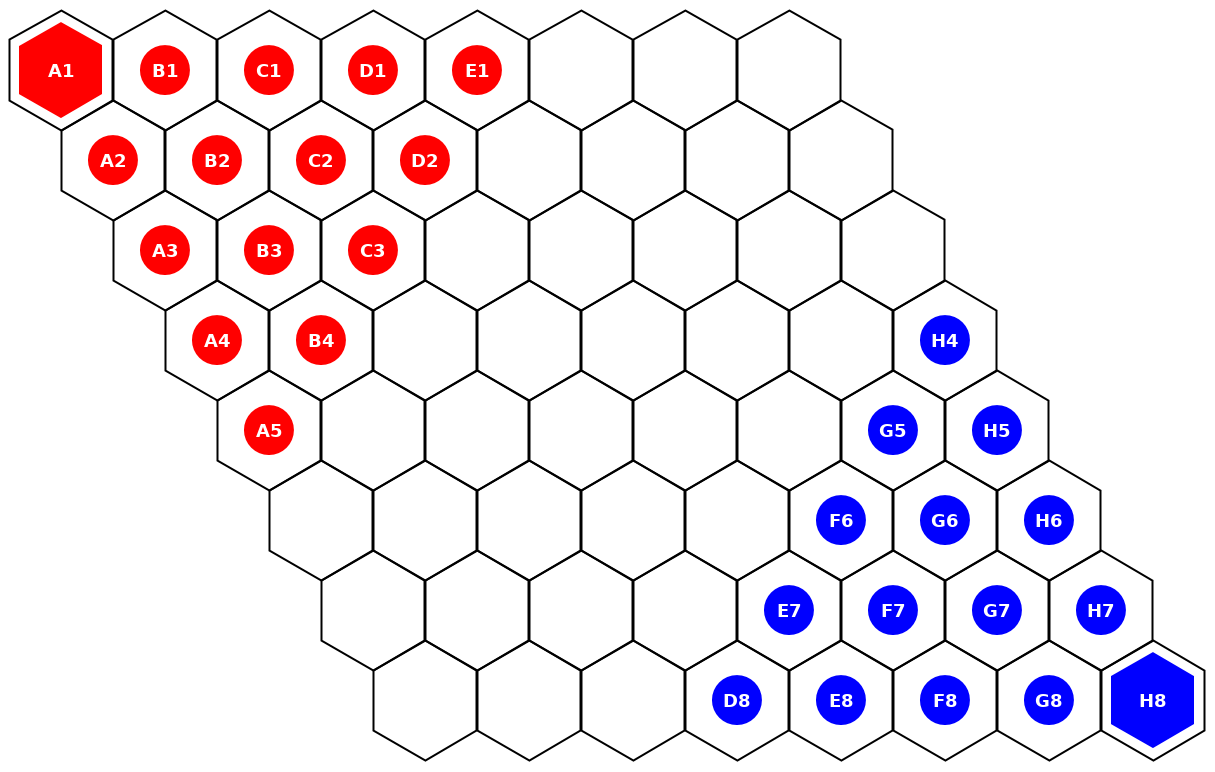
\includegraphics[scale=0.25]{graphic/start8.png}
\end{center}

Ein Nachbar eines Feldes ist ein Feld mit Abstand $1$ zu diesem. Jedes Feld in der Mitte hat demnach $6$ Nachbarn.

\subsection*{Spielablauf}
Der Spieler mit den roten Steinen hat den ersten Zug. Dann wird abwechselnd gezogen, einen Zug auszulassen ist nicht möglich. Ein Feld in TowerWarsPP ist entweder leer oder enthält eines der folgenden Elemente, deren Bedeutung gleich erklärt wird. In jedem Zug muss ein Spieler genau eine Figur von einem auf ein anderes Feld bewegen.

\subsubsection*{Basis}
Jeder Spieler hat zu Beginn des Spiels eine Basis, deren Position festgelegt ist. Diese kann nicht bewegt werden. Es ist auch nicht möglich eigene Figuren auf die eigene Basis zu bewegen.

Es ist Ziel des Spiels die gegnerische Basis zu zerstören und folglich auch die eigene zu verteidigen.

\subsubsection*{Steine}
Jeder Spieler hat zu Beginn eine vordefinierte Menge an Steinen. 

Ein Stein kann sich von sich aus ein Feld in jede Richtung bewegen (außer auf die eigene Basis natürlich).
\begin{figure}[ht]
\begin{center}
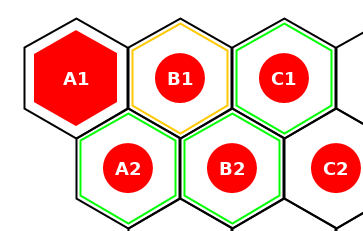
\includegraphics[scale=0.25]{graphic/token-nobase.png}
\end{center}
\caption*{$B1$ kann nicht auf Basis $A1$ ziehen}
\end{figure}

Zieht ein Stein auf ein leeres Feld, ist das ein ganz normaler Zug. Zieht ein Stein auf ein Feld mit einem gegnerischen Stein, ist dieser geschlagen und der eigene Stein nimmt dessen Platz ein.
\begin{figure}[ht]
\begin{center}
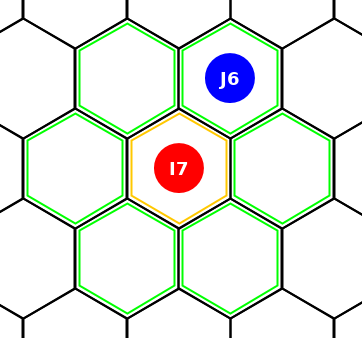
\includegraphics[scale=0.25]{graphic/token-move-kick.png}
\end{center}
\caption*{$I7$ kann auf ein benachbartes leeres Feld ziehen oder $J6$ schlagen}
\end{figure}

Ein Stein kann nicht auf die eigene Basis ziehen, sehr wohl jedoch auf die gegnerische Basis (was zum Sieg führt).
\newpage

\subsubsection*{Türme}
Türme haben eine Höhe $h \le h_\text{max}$, wobei \[h_\text{max} = \left\lfloor \frac{n}{3}\right\rfloor\]

Türme können geschlagen und \emph{blockiert} und Blockaden von Türmen können aufgehoben werden, dazu  später mehr.

\bigskip

Zu Beginn hat ein Spieler keine Türme. Türme können durch Ziehen eigener Steine auf eigene Steine gebaut und durch Ziehen eigener Steine auf Türme erhöht werden (falls dieser nicht bereits maximale Höhe hat). Es ist durchaus möglich ein Spiel ohne Bauen eines einzigen Turms zu spielen und zu gewinnen.

Zieht ein Stein auf ein Feld mit einem eigenen Stein, so wird auf diesem Feld ein Turm der Höhe $1$ gebaut.

Türme erhöhen die Reichweite angrenzender Steine um die Höhe des Turmes, dabei spielt es keine Rolle ob der Stein in dieser Reichweite Ziehen oder Schlagen will.

Hat ein Stein einen benachbarten Turm, so erhöht sich die Reichweite des Steins um die Höhe $h$ des Turmes. Der Stein kann dann auf alle erlaubten Felder mit Abstand $d \le 1 + h$ ziehen. Hat ein Stein mehrere angrenzende Türme, so summieren sich deren Höhen bei der Bestimmung der Reichweite auf. Blockierte Türme geben keinen Bonus. Ein Stein mit $6$ benachbarten Türmen kann folglich alle Felder mit folgendem Abstand erreichen \[d \le 1 + \sum_{i=1}^6 h_i\]

\begin{figure}[ht]
\begin{center}
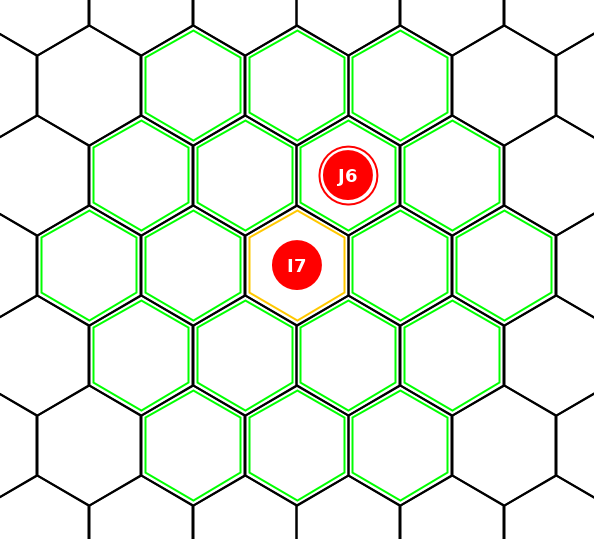
\includegraphics[scale=0.25]{graphic/move-ranged.png}
\end{center}
\caption*{$I7$ hat durch den Turm auf $J6$ die Reichweite $2$}
\end{figure}

\begin{figure}[ht]
\begin{center}
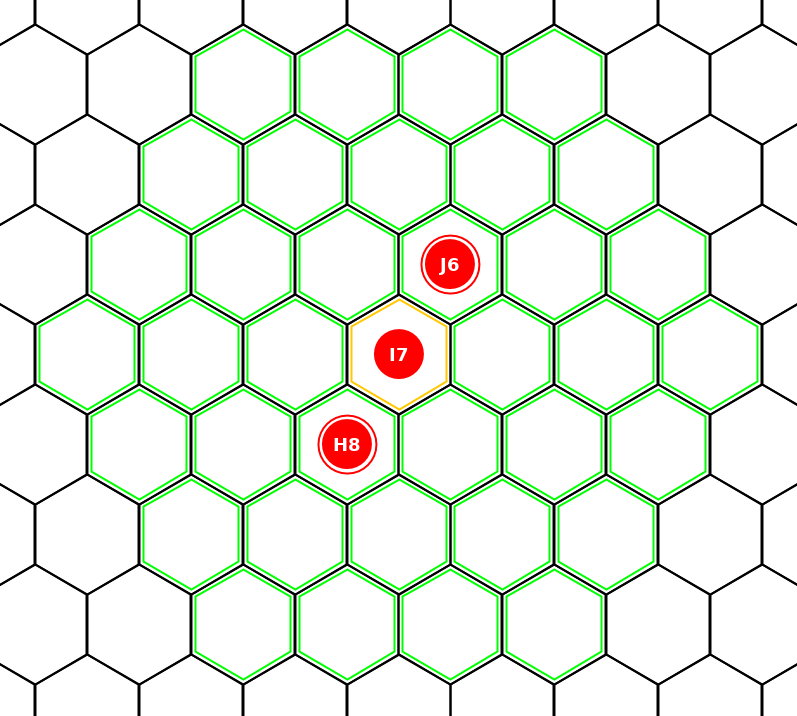
\includegraphics[scale=0.25]{graphic/move-rangeddouble.png}
\end{center}
\caption*{$I7$ hat durch die Türme auf $J6$ und $H8$ die Reichweite $3$}
\end{figure}

\begin{figure}[ht]
\begin{center}
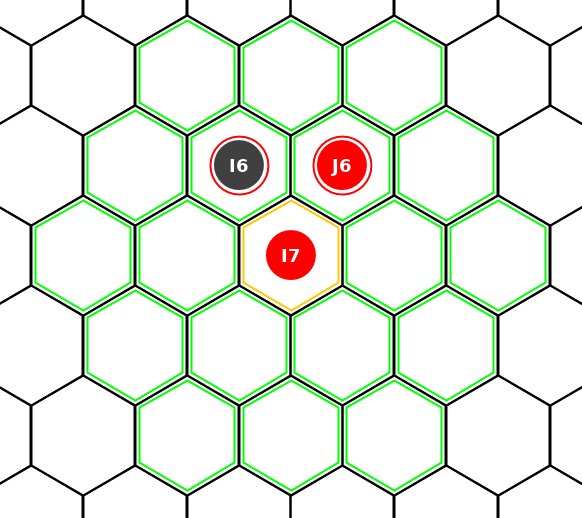
\includegraphics[scale=0.25]{graphic/range-blockedbonus.png}
\end{center}
\caption*{$I7$ hat einen Bonus durch Turm $J6$ aber nicht durch blockierten Turm $I6$}
\end{figure}

Zieht ein Stein auf ein benachbartes Feld spricht man von einem \emph{Nahzug}, sonst von einem \emph{Fernzug}.

\newpage
Zieht ein Stein auf ein Feld mit einem eigenen Turm, so wird dessen Höhe um $1$ erhöht (Ausnahme bilden hier blockierte Türme, deren Blockade aufgehoben wird und dessen Höhe unverändert bleibt). Hierbei darf die Maximalhöhe $h_\text{max}$ jedoch nicht überschritten werden.

\begin{figure}[ht]
\begin{center}
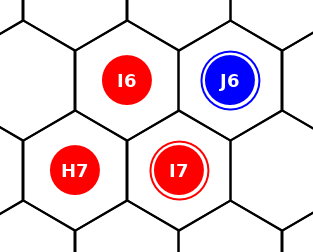
\includegraphics[scale=0.25]{graphic/token-kick-block-tower.png}
\end{center}
\caption*{$I6$ kann gegnerischen Turm $J6$ schlagen, $H7$ kann den gegnerischen Turm blockieren}
\end{figure}

Zieht ein Stein auf ein Feld mit einem gegnerischen Turm entscheidet die Art des Zuges was passiert. Handelt es sich um einen Nahzug, wird der gesamte gegnerische Turm geschlagen. Im Falle eines Fernzuges wird der gegnerische Turm blockiert.
\newpage

Auch Türme haben Zugmöglichkeiten. Es ist nicht möglich Türme in Ihrer Gesamtheit zu bewegen. 

Allerdings kann der oberste Stein vom Turm auf ein benachbartes Feld gezogen werden. Angrenzende Türme verleihen hierfür keinen Bonus auf die Reichweite. Es kann nur auf ein leeres oder eigenes Feld gezogen werden, ohne dabei die Maximalhöhe von Türmen zu überschreiten.

Bei diesem Abbau eines Turmes ist es nicht erlaubt zu schlagen. Daraus ergibt sich direkt, dass Türme nicht die gegnerische Basis schlagen können. Weiter ist es möglich, dass ein Spieler hierdurch keine Handlungsmöglichkeit mehr hat, wenn er nur noch einen Turm besitzt, der komplett von benachbarten gegnerischen Figuren besetzt ist. 

\begin{figure}[ht]
\begin{center}
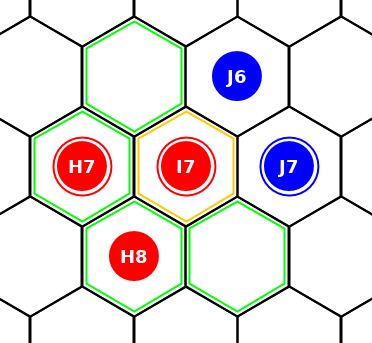
\includegraphics[scale=0.25]{graphic/tower-move.png}
\end{center}
\begin{itemize}
\item Turm $I7$ kann auf ein leeres Feld ziehen
\item Turm $I7$ kann auf den eigenen Stein $H8$ ziehen und damit einen neuen Turm bauen
\item Turm $I7$ kann auf den eigenen Turm $H7$ ziehen und diesen damit erhöhen
\item Turm $I7$ darf weder nach $J6$ noch nach $J7$ ziehen, da dort gegnerische Figuren stehen
\end{itemize}
\end{figure}

\begin{figure}[ht]
\begin{center}
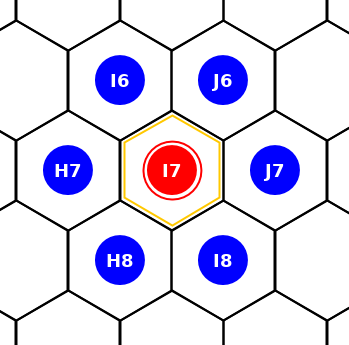
\includegraphics[scale=0.25]{graphic/neighbor-blocked-tower.png}
\end{center}
\caption*{Turm $I7$ hat keine Zugmöglichkeiten mehr}
\end{figure}

Beim Abbau des Turmes wird dessen Höhe natürlich um $1$ reduziert. Wird ein Turm der Höhe $1$ abgebaut, so bleibt dort ein normaler Stein zurück.

Ist ein Turm blockiert, kann dieser weder abgebaut werden noch gibt er anderen Steinen einen Bonus. Er steht nur noch blockiert auf dem Feld. 

Durch Ziehen eines eigenen Steins auf den Turm kann die Blockade wieder aufgehoben werden, ohne die Höhe des Turms zu verändern. Dies kann durch einen normalen Zug oder durch Abbau eines angrenzenden Turms auf diesen Turm erfolgen.
\newpage
\begin{figure}[ht]
\begin{center}
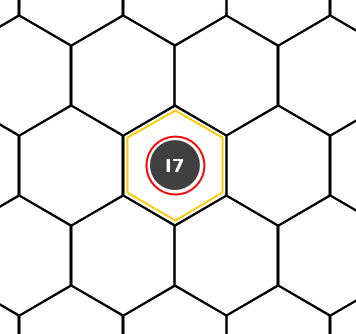
\includegraphics[scale=0.25]{graphic/tower-blocked.png}
\end{center}
\caption*{Turm $I7$ ist blockiert und kann nicht abgebaut werden}
\end{figure}

\begin{figure}[ht]
\begin{center}
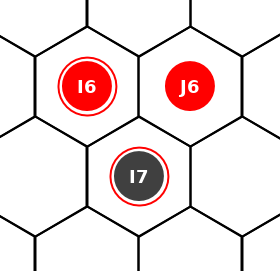
\includegraphics[scale=0.25]{graphic/tower-unblock.png} \\
\hspace{10pt}\\
Die Blockade von Turm $I7$ kann durch Abbauen des Turms $I6$\\ oder durch den Stein auf $J6$ aufgehoben werden
\end{center}
\end{figure}

\subsection*{Ende des Spiels}
Das Spiel ist gewonnen, wenn eine der folgenden Situationen eintritt:
\begin{itemize}
\item Ein Spieler zieht einen Stein auf die gegnerische Basis
\item Ein Spieler schlägt alle Steine des Gegenspielers
\item Ein Spieler macht den anderen Spieler handlungsunfähig
\item Der Gegenspieler gibt auf
\end{itemize}

Da in jedem Zug ein Stein bewegt werden muss und im Falle von keiner Zugmöglichkeit der Gegner gewinnt, kann das Spiel nicht unentschieden enden. Es ist jedoch sehr gut möglich, dass ein Spiel endlos andauert.

\subsection*{Spielidee}
Die Spielidee für TowerWarsPP wurde dieses Semester von Ole Umlauft und Dominick Leppich entwickelt und im Laufe von Testspielen zu dem ausgebaut, was jetzt in dieser Spielbeschreibung definiert ist.